\documentclass[11pt]{article}
\usepackage{graphicx}
\usepackage{bm}
\usepackage{amsmath}
\usepackage{amsfonts}
\usepackage{amssymb}
\usepackage{epsfig}
\usepackage{setspace}
\usepackage{dsfont}
\usepackage[shortlabels]{enumitem}
\usepackage{url}
\usepackage{color}
\usepackage[usenames,dvipsnames,svgnames,table]{xcolor}
\usepackage[authoryear,round]{natbib}
\usepackage[colorlinks = true, linkcolor = blue, citecolor = blue, citecolor = blue]{hyperref}
\usepackage{tikz}
\usepackage{pgfplots}
\usepackage{subcaption}
\usepackage{verbatim}
\usepackage{caption}
\usepackage{booktabs}
\usepackage{longtable}
\usepackage{array}
\usepackage{float}
\usepackage{pdflscape}
\usepackage[utf8]{inputenc}
\usepackage[english]{babel}
\usepackage{xcolor}
\usepackage{comment}
\usepackage{indentfirst}
\usepackage{setspace}
\usepackage{soul}
\usepackage[normalem]{ulem}
\usepackage{epigraph}

\usetikzlibrary{automata,arrows,positioning,calc}
\usetikzlibrary{plotmarks}
\usetikzlibrary{decorations.pathreplacing}

\addtolength{\voffset}{-1.5cm} \addtolength{\hoffset}{-1cm}
\addtolength{\textwidth}{2.5cm} \addtolength{\textheight}{2.5cm}

\newtheorem{hypothesis}{Hypothesis}


\pgfplotsset{compat=1.17}
\renewcommand{\baselinestretch}{1.5}

%%%%%%%%% Path resolution (Overleaf: tables/, plots/; Local: ../output/) %%%%%%%%%
\graphicspath{{plots/}{../output/plots/}}
\makeatletter
\def\input@path{{tables/}{../output/tables/}}
\makeatother

%%%%%%%%%%%%%%%%%%%%%%%%%%%%%%%%%%%%%%%%%%%%%%%%


\title{To Sell or not to Sell:\\ The Psychology of Market Runs%\thanks{Grant number xxx, IRB number xxx, We thank}
}


\author{Caleb Eynon\thanks{University of Alabama, ceynon@crimson.ua.edu} 
~and  Paan Jindapon\thanks{University of Alabama, pjindapon@ua.edu}  }



\date{\today}

\begin{document}

\maketitle


\section*{\centering\textbf{Abstract}}
\noindent
\begin{singlespace}

\noindent
We investigate the psychological predictors of market runs in an experimental setting. Specifically, we examine the effect of emotions, personality traits, luck, communication, and peer liquidation on the probability of a run occurring in a financial market. We conduct a laboratory experiment with a 2x2 design, varying the liquidation value distribution and the availability of pre-play communication. The participants act as investors with incentive to beat the market by preempting other investors when the fundamental value of an asset is sufficiently low. We use facial reading technology and surveys to measure emotions and personality traits among participants during the experiment. We find that traits and emotions associated with worry or negativity increase the likelihood of an investor entering a market run while investors that get ``lucky'' are less likely to sell in subsequent markets. We find evidence for cascade effects, investors quickly selling after each other. Finally, we find that anxiety decreases welfare in the market. Our results suggest that individual psychological factors and reactions to non-fundamental events are significant predictors of participation in financial market runs. 

\end{singlespace}
\newpage






\epigraph{``Until you can manage your emotions, don’t expect to manage money.''}{\textit{-Warren Buffett}}



%%%%%%%%%%%%%%%%%%%%%%%%%%%%%%%%%%%%%%%%%%
\section{Introduction}
%%%%%%%%%%%%%%%%%%%%%%%%%%%%%%%%%%%%%%%%%%

Financial volatility has been a concern since the inception of markets\footnote{See, for example, the Dutch Tulip Bulb Crisis of 1630}. Panic induced liquidation has been a symptom of recent financial crises. For example, in March 2020 the Dow Jones Industrial Average fell by 26\% in just four days at the beginning of the COVID recession. Another example is Black Monday in 1987, when the Dow Jones Industrial Average fell by 22.6\% in just one day. While much of the subsequent drops in prices were based on fundamentals of the economy, there is debate as to how much investors overreact to bad economic news. \cite{thaler1985} shows that most people overreact to unexpected and dramatic news events in a financial market setting. 

Ever since \cite{diamond1983bank}, the seminal paper on bank runs, the literature on financial runs has largely focused on bank runs. Market runs, defined as situations where investors fear having to liquidate shares after a run, but before prices can recover back to fundamental values, differ from bank runs in several ways \citep{bernardo2004liquidity}. First, the source of fragility for a bank run comes from the investment in long terms assets and then too many depositors seeking to withdraw before the return can be realized. However, the source of fragility in market runs is the liquidity of the market, the demand for shares on the buy side. Second, each withdrawal in a bank run depletes an asset pool which can pay out full deposits until it is depleted. In the market run setting, each sale immediately impacts price, so order of sale matters for the price received by an investor. Finally, and arguably most importantly, the model of bank runs allows for deposit insurance to prevent the run equilibrium, whereas this is impossible in the model of market runs. This is because deposits have an easily observable fundamental value, but it can be difficult to determine the fundamental value of an asset. Additionally, the Bayesian belief about fundamental value of the asset changes as signals are added. Therefore, it is important to study the drivers of these market runs, and what solutions are available to combat instability.

It is of interest to policymakers and economists to determine what might cause overreactions to unexpected and dramatic news, specifically the psychological aspect. \cite{bracha2012psychological} proposes a psychological account of financial panics in which a rational slow system competes with a fast emotional system. We use an experimental approach to test which emotions and personality traits predict the sale of assets in a financial market, specifically, a market where runs are possible. We also test other panic-inducing factors such as unluckiness and cascade effects. By understanding the factors that contribute to overreactions in financial markets, businesses and governments can be better prepared with tools to prevent panic and financial instability.

We set up an environment consistent with \cite{bernardo2004liquidity}, where investors face some liquidity need in the future and own an asset. They can hold this asset until an uncertain terminal period or sell at any time prior. If the state of the world is bad, then the investor must sell their asset at the market price at the terminal period; whereas in the good state of the world, investors can earn some long term rate of return at the terminal period. Investors observe public, stochastic signals about the state of the world as time goes on, with the Bayesian probability almost surely converging to 1 for the true state. In the good state, investors have incentive to hold until the terminal period, but in the bad state, investors have incentive to preempt other investors by selling before them. These sales generate a negative externality for other investors, lowering the liquidation price of their asset. Since players do not know the state of the world ex ante, if the signal is sufficiently bad, equilibrium is when the investors run on the market. Since these signals are stochastic, there will be some good state markets that end in a market run because of a poor start for the signal. This ultimately decreases welfare for investors. %This is a similar set up to \cite{magnani2020dynamic} and \cite{choi2022market}.

Importantly, investors can observe the signal, price, and sales in the asset market in order to inform their selling decision. In an experimental setting, this allows us to set up facial recognition technology to observe investor emotions prior to sales while they use the information to make their decision. In addition to creating an environment where observing emotions is possible, we also add treatments to the experiment to assess other factors in market runs. We implement a treatment where liquidation payoffs are decided randomly vs averaged across remaining investors. In the average treatment, investors may feel more cooperative since they are guaranteed the same liquidation value at the terminal period if they don't sell prior to that. This allows us to test whether this joint sense of responsibility can help reduce the occurrence of market runs. Additionally, we introduce communication in some markets. This provides a different approach to cooperation, allowing investors to potentially derive a strategy or reassure each other. This can help determine if communication channels, such as online chat rooms, could decrease the occurrence of market runs.

We implement an experiment consistent with what is listed above. Our experiment compares markets in a mixed design settings, where liquidation payoffs are between subjects and market communications are within subjects. We then derive hypotheses based on the model put forth by \cite{bernardo2004liquidity} and first placed in an experimental setting by \cite{magnani2020dynamic}.

We contribute to the literature by bridging a gap between bank run psychology and market run psychology. To our knowledge, we are the first to measure emotions as they relate to investors in this market run model. Additionally, we add to the literature detailing financial behavior as it relates to personality traits. Finally, we contribute to the literature on cascading and herding effects in financial markets. 

We find evidence of several factors that affect an investor's likelihood to sell her asset. First, cascade effects are present, a different investor selling in a time period very shortly before the current one causes an increase in the likelihood of selling for other investors. Second, an investor receiving an ``unlucky'' liquidation payoff in the bad state is much more likely to sell in a future market than an investor that received a ``lucky'' payoff in the same exact market. Third, emotions that are typically associated with worry or negativity are positive predictors of an investor selling. Finally, certain time-invariant personality traits cause an increase in selling probability while one trait, risk tolerance\footnote{As measured using an version of the method proposed by \cite{gneezy1997experiment}.}, causes a decrease in selling probability.

The remainder of the paper is organized as follows. In section 2, we summarize the relevant literature. In section 3, we describe our experimental design and market model. In section 4, we state our hypotheses. Section 5, presents the results from the experiment. Section 6 discusses the results and concludes. 

%%%%%%%%%%%%%%%%%%%%%%%%%%%%%%%%%%%%%%%%%%
\section{Related Literature}
%%%%%%%%%%%%%%%%%%%%%%%%%%%%%%%%%%%%%%%%%%

\subsection{Market Runs Experiments}

\cite{bernardo2004liquidity} provides the original theoretical background for our experiment. They model runs in financial markets similar to bank runs. Importantly, each risk neutral investor has incentive to beat the market by selling before other investors. Investors fear being forced to sell at the post run price and each investor prefers to sell early to avoid the possibility of being stuck on the wrong side of a run. This causes runs to be caused by the fear of future liquidity shocks. \cite{magnani2020dynamic} is the first paper to implement this model experimentally. They specifically look at a ``circuit-breaker'' policy as a potential intervention to stop market runs and restore stability in some cases. They find that circuit-breakers are effective when information quality is high enough, otherwise the break in trading does not aggregate enough information for seller behavior to change. \cite{choi2022market} also implements this model experimentally. They examine the role of liquidity in investor sensitivity to information. They find that lower liquidity markets are more susceptible to over-sensitivity and that herding behavior is more prominent. 




\subsection{Bank Runs Experiments}

As mentioned in Section 1, market runs are related to bank runs. \cite{diamond1983bank} provide the original theory for bank runs, demonstrating that coordination failure among depositors can lead to runs. Several papers implement their model in an experimental setting. \cite{madies2006experimental} studies a static model and find that bank runs are persistent. \cite{garratt2009bank} show that bank runs are more likely to occur in environments where there is significant uncertainty about fundamental withdrawal demand and depositors receive information about the behavior of other depositors when there are multiple opportunities to withdraw. In particular,  uncertainty regarding the number of impatient depositors increases the likelihood of a bank run.  \cite{schotter2009dynamics} show that depositors are willing to restrain themselves from withdrawing when they can learn from additional information and the existence of an insider who has informational advantage exists can delay the decision to withdraw.



\cite{kiss2014social} and \cite{kiss2018panic} focus on observability of other player's action. \cite{chakravarty2014experiment} and \cite{brown2017understanding} design experiments with two banks and examine bank-run contagion. They find that withdrawals on one bank can trigger panic bank-run at another bank despite liquidity independence between the two banks.

Two papers implement analyses similar to ours. First, \cite{dijk2017bank} induces fear, sadness, or happiness in each treatment in an emotional task prior to playing the game. They find that the inducement of fear causes a large increase in the probability of withdrawal and subsequent run. While we also examine an emotional effect, we do not induce the emotion but rather use software recognize emotions as they occur throughout the experiment. \cite{shakina2018coordination} use chat and no-chat between-subjects treatments and find that communication, especially positive messages, can slow down withdrawals. While we also use chat and no-chat treatments, we do it within-subjects. 



\subsection{Psychological Factors}



Neuroticism is related to attitudes towards risk, with higher neuroticism associated with lower risk tolerance \citep{rustichini2016toward}.  \cite{oehler2018investors} find that extraverted individuals are willing to pay higher prices for financial assets and more neurotic individuals hold less risky assets. \cite{de2019personality} find that people who have a high degree of openness to experience have the greatest probability of taking higher levels of risk in their investment decisions.



Using a questionnaire based on the State-Trait Anger Expression Inventory (STAXI) and the State-Trait Anxiety Inventory (STAI), \cite{gambetti2012effect} find that trait anger is positively associated with the willingness to invest in risky assets, while trait anxiety predicts conservative financial decisions. Using the Sixteen Personality Factor (16PF) questionnaire, \cite{gambetti2019personality} also find that anxious people tend to save money and avoid investments.



\cite{cecchini2019individual}  find that, as an asset price in increasing,  extroverted subjects sell the asset too quickly while conscientious subjects are more patient and sell the asset at a higher price. \cite{bajo2023psychological} also find a significant effect of  conscientiousness in explaining higher trading volume and greater risk taking.





%\cite{nyhus2001role}
%\cite{donnelly2012big}
%\cite{brown2014household}
%\cite{tauni2020investor}
%\cite{barratt1959anxiety}
%\cite{fowles1987application}
%\cite{whiteside2001five}
%\cite{verplanken2001individual}
%\cite{gathergood2012self}
%\cite{ottaviani2011impulsivity}
%\cite{friederich2024crypto}









%%%%%%%%%%%%%%%%%%%%%%%%%%%%%%%%%%%%%%%%%%
\section{Design of the Experiment}
%%%%%%%%%%%%%%%%%%%%%%%%%%%%%%%%%%%%%%%%%%
We experimentally implement the \cite{bernardo2004liquidity} framework in a laboratory setting. Our implementation is similar to that of \cite{magnani2020dynamic} and \cite{choi2022market}.

\subsection{Market Model} \label{sec:market model}
There are two types of agents in a market, a risk averse market-maker and risk-neutral individual investors. Each investor is endowed with a unit of an asset. There are $N=4$ investors\footnote{For a more general representation of the market model, see \cite{magnani2020dynamic}.} in each market. The market-maker is willing to absorb these assets upon demand. The market lasts for $T \in \mathbb{N}$ discrete time periods. Each investor has the choice to sell their asset in any discrete period $t < T$, but cannot repurchase, making the decision to sell final for that investor in the market. $T$ is a random variable following a geometric distribution with probability of termination $\lambda = 0.125$.

There are two possible states of the world, good and bad. In the good state, any investor that still holds their asset at time $T$ receives the asset's ``final value'', $v$ ,which is interpretable as an asset return. In our case, $v=20$. This \textit{does not} depend on the number of market participants that have not sold their asset. In the bad state, investors face a liquidity shock at time $T$ and are forced to sell their asset at the market price.

The market price is determined by a price schedule. Let $p_n$ be the market price of the asset when $n$ investors have not yet sold their asset. Then, $ v > p_4 > p_3 > p_2 > p_1$, meaning that a sale causes a fall in price, consistent with illiquidity. \cite{bernardo2004liquidity} show that the price schedule can be derived as linear with the assumption of a risk-averse competitive market-maker. Thus, we use the following price schedule $p_n = 8 - 2(4-n)$. In the event that multiple investors sell in period $t$, then the investors are randomly ordered with equal probability and receive the associated sale prices.

The state of the world is uncertain. Let $z$ be the state of the world and G and B represent the good and bad states respectively. Each investor in a market begins with the common belief\footnote{We define $\pi(t)$ slightly differently that \cite{magnani2020dynamic}. This is done to allow $\pi(t)$ to converge to 1 in the good state, which is more representative of our experimental implementation.}  $\pi(0) := P(z = G) = 0.5$. At the beginning of a period $t$, each investor receives a binary public signal ($y(t)$, good ($y(t) = g$) or bad ($y(t) = b$). The likelihood of each signal depends of the quality of information. In our implementation, we use the HIGH information quality state from \cite{magnani2020dynamic} which sets $\mu_B = P(y(t) = b | z = B) = 0.675$ and $\mu_G = P(y(t) = g | z = B) = 0.325$. Thus, each investor's belief in period $t$ via Bayesian updating is
\begin{equation}
    \pi(t) := P(z = G|y(t), \pi(t-1)) =
    \begin{cases}
        \frac{\pi(t-1)(1-\mu_B)}{\pi(t-1)(1-\mu_B) + (1-\pi(t-1))\mu_B}, & \text{if   } y(t) = b \\
        \frac{\pi(t-1)(1-\mu_G)}{\pi(t-1)(1-\mu_G) + (1-\pi(t-1))\mu_G}, & \text{if   } y(t) = g
    \end{cases}
    \label{eq:bayes}
\end{equation}

$\pi(t) \overset{a.s.}{\to} 1$ if the state of the market is good and $\pi(t) \overset{a.s.}{\to} 0 $ if the state of the market is bad.
This model captures key components of a market run environment.
\begin{itemize}
    \item Investors can rapidly sell their assets and can do so at a time of their choosing.
    \item There is uncertainty to the true state of the market that accrues over time.
    \item Investors have incentive to sell before their market counterparts if the state of the market is bad.
\end{itemize}

\subsection{Investor Welfare}

We now show that early liquidations decrease investor welfare when $z = G$. Define investor welfare as the ratio of total utility
received by investors to the maximum total possible utility received by investors. Let $u(\cdot)$ be a generic utility function. When $z=B$, the maximum total possible utility is $\sum_{n=1}^{4} u(p_n)$
since each investor will either voluntarily sell during the market or be forced to sell at the terminal period. When $z=G$, the maximum possible total utility is $4 \cdot u(v=20)$ since each investor cannot sell
their asset during the market for any more than $p_4=8$. Thus welfare when $z=B$ is given by,
\begin{equation}
  w_m = \dfrac{\sum_{n=m+1}^{4} u(p_n) + \sum_{n=1}^{m} u(p_n)}{\sum_{n=1}^{4} u(p_n)} = 1 \; \forall m \in \{0,1,2,3,4\}
  \label{eq:welfare_bad}
\end{equation}
where $m$ is the number of participants that do not sell their asset during the market. In the bad state, welfare is always maximized. When $z=G$, the welfare function is,

\begin{equation}
  w_m = \dfrac{\sum_{n=m+1}^{4} u(p_n) + m\cdot u(v=20)}{4 \cdot u(v=20)} \le 1 \; \forall m \in \{0,1,2,3,4\}
  \label{eq:welfare_good}
\end{equation}

Suppose that $u(\cdot)$ is CRRA, with $u(p_n) = \dfrac{p_n^{1-\alpha}}{1-\alpha}$. Then we can examine the relationship between risk aversion and welfare
in each of the five cases of $m$. Figure \ref{fig:welfare} plots each welfare possibility against risk aversion, $\alpha$. Since $z=G$, welfare is maximized
when $m=4$ and minimized when $m=0$. The differences in welfare for each scenario are largest when investors are risk neutral ($\alpha = 0$). The differences
are the smallest when investors are risk averse ($\alpha \rightarrow 1$). This can be interpreted as investors gaining some utility from becoming certain about
their payoff earlier in the market.

\subsection{Best Replies and Equilibrium}

\begin{figure}
  \centering
  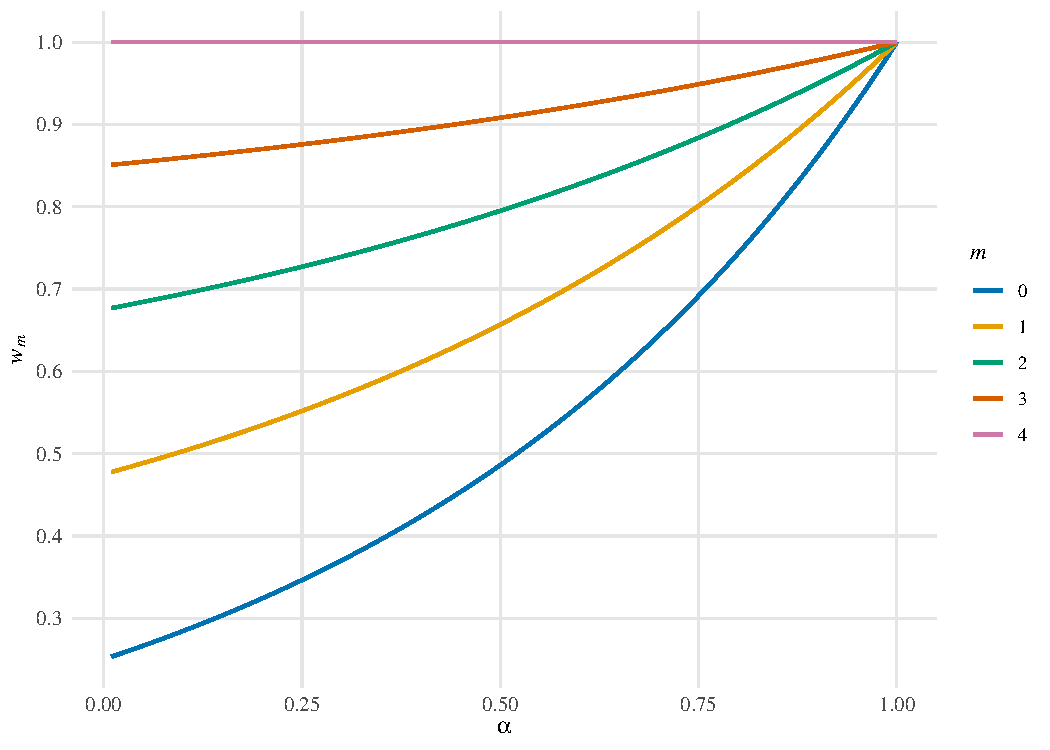
\includegraphics[width=0.8\linewidth]{welfare_theory.pdf}
  \caption{Welfare of each possible ending market scenario as it relates to risk aversion, $\alpha$.}
  \label{fig:welfare}
\end{figure}

\begin{figure}
  \centering
  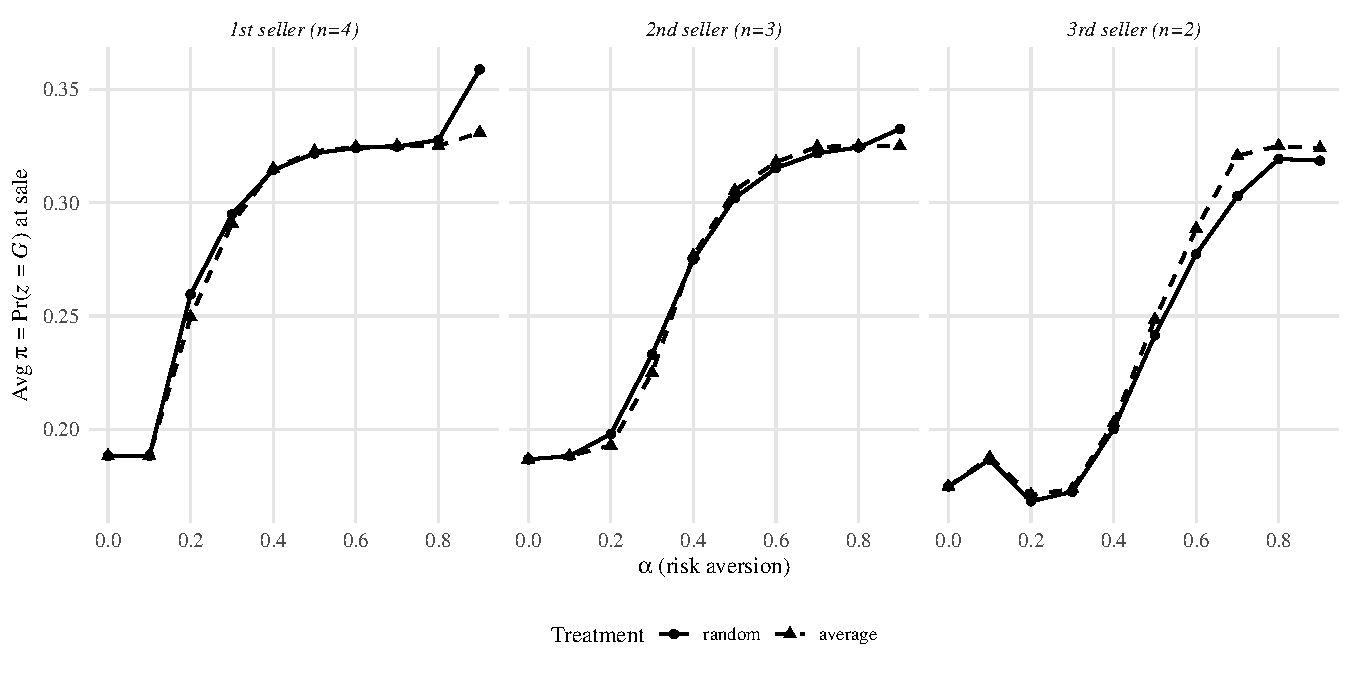
\includegraphics[width=\linewidth]{equilibrium_avg_pi_at_sale.pdf}
  \caption{Average equilibrium belief $\pi = \Pr(z=G)$ at sale by seller position across risk aversion levels. Solid lines (circles) represent Treatment~1 (Random) and dashed lines (triangles) represent Treatment~2 (Average). The treatment gap widens with risk aversion, consistent with the variance-reduction channel of the Average payoff scheme. Numerical values are reported in Table~\ref{tab:equilibrium_thresholds}.}
  \label{fig:avg_pi_at_sale}
\end{figure}

\subsection{Experimental Implementation}
We conducted six experimental sessions, each with 16 subjects in the TIDE Lab at the University of Alabama. Subjects were students at the university ranging in age from 18 to 34. Each session consisted of three parts, first subjects privately watched an instructions video and completed a quiz\footnote{The average quiz score on the first attempt across all six sessions was 85.7\%.} on their computer with headphones\footnote{A typed version of the video is available in \ref{sec:app_instr}, and the video can be found in the online appendix.}. Subjects answered the questions independently first, then the correct answers were read aloud by the experimenters. Then subjects proceeded to complete part 1, the market portion, of the experiment. Following, the conclusion of part 1, subjects completed part 2, the survey portion.
Each participant was assigned an alphabet letter as an identifier that was constant throughout the session. Each entire session consisted of 4 segments. At the beginning of each segment, participants were grouped into four groups of four. Each segment grouping was designed such that no two participants are grouped together more than once. At the beginning of segments 1 and 2, participants did not interact with each other. At the beginning of segments 3 and 4, participants could communicate with members of their group through a virtual chat environment for 90 seconds.

Each segment consisted of an uncertain number of rounds, equivalent to a market as described in \ref{sec:market model}. The number of rounds was randomly generated prior to the experiment according to a geometric distribution with probability of termination equal to $0.125$. Participants were not regrouped in between rounds. This allows us to observe within-group variation across markets. At the beginning of each market (round), each participant was endowed with an asset and their initial belief about the state was set to 0.5, so $\pi(0) = 0.5$. Figure~\ref{fig:experiment_flow} summarizes the hierarchical structure of a session.

% Experiment flow diagram: hierarchical tree showing session structure
% Session -> Segments -> Rounds -> Periods
% Uses TikZ libraries: automata, arrows, positioning, calc (loaded in main.tex)

\begin{figure}[H]
\centering
\resizebox{\textwidth}{!}{%
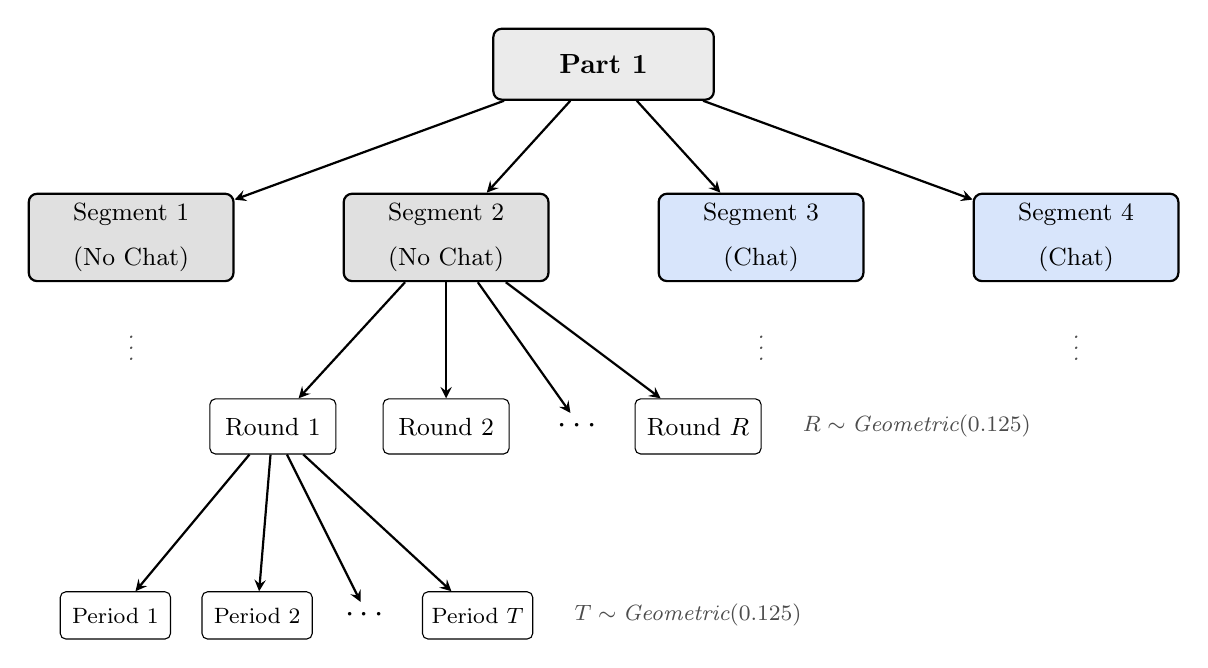
\begin{tikzpicture}[
    % Node styles
    session/.style={
        rectangle, draw, thick, rounded corners=3pt,
        fill=black!8, minimum width=2.8cm, minimum height=0.9cm,
        font=\bfseries\normalsize
    },
    nochat/.style={
        rectangle, draw, thick, rounded corners=3pt,
        fill=black!12, minimum width=2.6cm, minimum height=0.8cm,
        font=\small, align=center
    },
    chat/.style={
        rectangle, draw, thick, rounded corners=3pt,
        fill=CornflowerBlue!25, minimum width=2.6cm, minimum height=0.8cm,
        font=\small, align=center
    },
    roundnode/.style={
        rectangle, draw, rounded corners=2pt,
        fill=white, minimum width=1.6cm, minimum height=0.7cm,
        font=\small
    },
    periodnode/.style={
        rectangle, draw, rounded corners=2pt,
        fill=white, minimum width=1.4cm, minimum height=0.6cm,
        font=\footnotesize
    },
    ellipsisnode/.style={
        font=\large, inner sep=2pt
    },
    annotation/.style={
        font=\footnotesize\itshape, text=black!70
    },
    arrowed/.style={
        ->, >=stealth, thick
    },
]

% === Session node ===
\node[session] (session) {Part 1};

% === Segment nodes (evenly spaced using absolute x-coordinates) ===
\node[nochat] (seg1) at (-6, -2.2) {Segment 1\\(No Chat)};
\node[nochat] (seg2) at (-2, -2.2) {Segment 2\\(No Chat)};
\node[chat]   (seg3) at ( 2, -2.2) {Segment 3\\(Chat)};
\node[chat]   (seg4) at ( 6, -2.2) {Segment 4\\(Chat)};

% === Session -> Segment edges ===
\draw[arrowed] (session) -- (seg1);
\draw[arrowed] (session) -- (seg2);
\draw[arrowed] (session) -- (seg3);
\draw[arrowed] (session) -- (seg4);

% === Vertical dots under segments without expanded subtree ===
\node[annotation] at (-6, -3.5) {$\vdots$};
\node[annotation] at ( 2, -3.5) {$\vdots$};
\node[annotation] at ( 6, -3.5) {$\vdots$};

% === Round nodes (under Segment 2) ===
\node[roundnode] (r1) at (-4.2, -4.6) {Round 1};
\node[roundnode] (r2) at (-2.0, -4.6) {Round 2};
\node[ellipsisnode] (rdots) at (-0.3, -4.6) {$\cdots$};
\node[roundnode] (rR) at (1.2, -4.6) {Round $R$};

% === Segment -> Round edges ===
\draw[arrowed] (seg2) -- (r1);
\draw[arrowed] (seg2) -- (r2);
\draw[arrowed] (seg2) -- (rdots);
\draw[arrowed] (seg2) -- (rR);

% === Geometric annotation for rounds ===
\node[annotation, right=0.4cm of rR]
    {$R \sim \text{Geometric}(0.125)$};

% === Period nodes (under Round 1) ===
\node[periodnode] (p1) at (-6.2, -7.0) {Period 1};
\node[periodnode] (p2) at (-4.4, -7.0) {Period 2};
\node[ellipsisnode] (pdots) at (-3.0, -7.0) {$\cdots$};
\node[periodnode] (pT) at (-1.6, -7.0) {Period $T$};

% === Round -> Period edges ===
\draw[arrowed] (r1) -- (p1);
\draw[arrowed] (r1) -- (p2);
\draw[arrowed] (r1) -- (pdots);
\draw[arrowed] (r1) -- (pT);

% === Geometric annotation for periods ===
\node[annotation, right=0.4cm of pT]
    {$T \sim \text{Geometric}(0.125)$};

\end{tikzpicture}%
}% end resizebox
\caption{Hierarchical structure of the experiment.}
\label{fig:experiment_flow}
\end{figure}


In the market portion of the session we use a mixed design with 2 between-subjects treatments and 2 within-subjects treatments. The within subjects treatment was the ability to chat with other market participants. In the first two segments of the experiment, no chat was permitted between participants. In the last two segments, participants were permitted to communicate with each other in a virtual chat environment prior to the start of each segment. This allows us to understand the emotions and thoughts of participants even further. We used a within-subjects design as to prevent bias associated with chat in a between-subjects design. For example, in a between-subjects treatment, participants would either take a vastly different amount of time to go through the experiment, or some participants would have to experience some amount of ``dead time'' without communication.

In treatment 1, each of these markets followed the game described in \ref{sec:market model}. In treatment 2, the price schedule was modified in the event that multiple market participants sold in the same time period $t$. Suppose there are $N$ participants still holding their asset at time $t-1$ and $M \in \{1,2,...,N\}$ market participants sell in time period $t$. Then in treatment 2, each market participant who sold in $t$ receives \begin{equation}
    \bar{p}_{N,M} = \dfrac{\sum_{m=1}^M p_{N-m+1}}{M}
\end{equation}

This modification includes the case where the bad state of the market forces liquidation at the terminal period $T$. Let $P_{i,t,N,M}$ be the set of payoffs when $M$ participants sell their assets in period $t$ in treatment $i$ when $N$ participants still held their asset in $t-1$. Then
\begin{equation}
    E(P_{1,t,N,M}) = E(P_{2,t,N,M}) \; \forall \, t\in\{1,2,...,T\}, N \in \{1,2,3,4\},M \in \{1,...,N\}
\end{equation}
\begin{equation}
    Var(P_{1,t,N,M}) \ge Var(P_{2,t,N,M}) \; \forall \, t\in\{1,2,...,T\}, N \in \{1,2,3,4\},M \in \{1,...,N\}
\end{equation}
Note that $Var(P_{2,t,N,M}) = 0 \; \forall \, t\in\{1,2,...,T\}, N \in \{1,2,3,4\},M \in \{1,...,N\}$

Each subject only participated in one treatment. Of our six experimental sessions, three were treatment 1 and three were treatment 2.

At the beginning of each period within a round, each market participant could see $p_N$ and all previously market prices, $\pi(t)$ which has been calculated for them\footnote{This slightly differs from \cite{magnani2020dynamic} who do not compute the Bayesian updated probabilities for participants.} using Equation \ref{eq:bayes}, market participants who have sold, a ``SELL'' button, and their price received (if applicable). See Figure \ref{fig:interface}. Each period lasted 4 seconds. The number of periods in each round was randomly determined prior to the experiment, but the sequence of signals was randomly determined in real time.

\begin{figure}
    \centering
    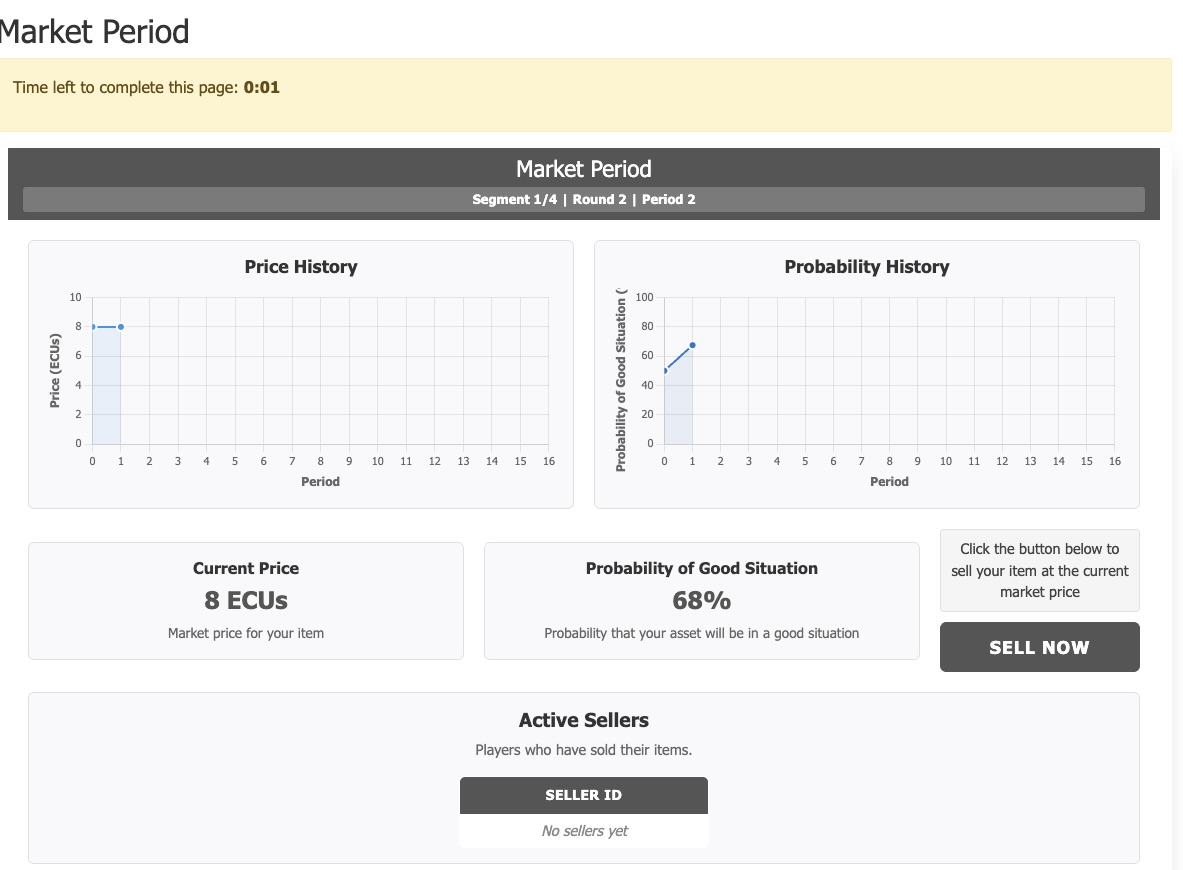
\includegraphics[width=0.8\linewidth]{interface.jpeg}
    \caption{An example of the participant market period interface}
    \label{fig:interface}
\end{figure}

At the conclusion of a round, each participant was shown the true state of the market, the price they received, the current segment number, and current round number. The break in between rounds lasted 15 seconds.

Following the conclusion of segment 2, participants were informed that they would be able to communicate with market participants prior to the start of each segment. They also received a set of rules restricting the use of profanity or the disclosure of identifying information. Other than that, participants were free to chat about any topic that they wished.

Following the conclusion of segment 4, participants move onto the survey portion of the experiment. Like \cite{gutsche2023determinants}, we use the Ten Item Personality Inventory (TIPI) according to \cite{gosling2003very} to capture these five personality traits. The resulting variables ‘extraversion,’ ‘agreeableness,’  ‘conscientiousness,’ ‘neuroticism,’ and ‘openness to experiences’ range between one and five, with a higher value associated with a higher degree of the corresponding personality trait.  We elicited individual risk preferences using a task similar to \cite{gneezy1997experiment}. Each participant received 20 points and decided how much to invest in a risky option. The risky option had a 50\% chance of success. If the investment failed, the participant lost the invested amount; if successful, the payoff was 2.5 times the invested amount. 

At the conclusion of the survey portion, each participants earnings were calculated. They received $\$7.50$ as a participation fee plus their earnings from part 1 plus their earnings from part 2. For part 1, one market from each segment was randomly selected and then summed. Participants were not aware of the selected market from each segment until the conclusion of part 2. For part 2, participants receive 20 ECU's for completing the survey questions, and then have the opportunity to gamble those earnings in the risk aversion task. Earnings from part 1 and 2 were then converted at the rate of 4 Experimental Currency Units (ECU's) to \$1. Earnings from all six sessions ranged from \$11.00 to \$36.25 with a mean of \$23.57. Each session lasted approximately 75 minutes.

\begin{table}[H]
  \centering
  \caption{Pre-randomized experimental parameters by segment}
  \label{tab:randomized_params}
  \begingroup
\centering
\small
\begin{tabular}{cccccc}
\toprule
Segment & Chat & Rounds & Periods per Round & Total Periods & Avg. per Round \\
\midrule
  1 & No & 10 & 3, 10, 8, 4, 2, 3, 9, 7, 4, 6 & 56 & 5.6 \\
  2 & No & 5 & 9, 2, 5, 6, 5 & 27 & 5.4 \\
  3 & Yes & 6 & 9, 8, 4, 4, 3, 5 & 33 & 5.5 \\
  4 & Yes & 9 & 5, 3, 11, 3, 6, 14, 6, 3, 1 & 52 & 5.8 \\
\midrule
 \multicolumn{2}{c}{Total}  & 30 & --- & 168 & --- \\
 \multicolumn{2}{c}{ Avg. per Segment} & 7.5 & --- & 42.0 & 5.6 \\
\bottomrule
\end{tabular}
\endgroup

\end{table}

\subsubsection{A Liquidation Example, Treatment 1 vs. Treatment 2}
Suppose that we are in a market with four participants. Suppose at time $t-1$, no market participant has sold. Then in period $t$, both participants A and B decide to sell their asset. In treatment 1, according to our specified price schedule, A receives $p_4 = 8$ with probability 0.5 and $p_3 = 6$ with probability 0.5. B then receives whichever price A does not. In treatment 2, both A and B would receive $\bar{p}_{4,2} = (p_4+p_3)/2 = (8+6)/2 = 7$.

Now suppose that in period $t$, participants A, B, and C decided to sell their asset (as opposed to just A and B). In treatment 1, each participant would be assigned a price from the schedule $\{p_4=8,p_3=6,p_2=4\}$ with exclusivity. In treatment 2, participants A, B, and C would each receive $\bar{p}_{4,3} = (p_4+p_3+p_2)/3 = (8+6+4)/3 = 6$.

Finally, suppose that in period $t$, just participant A decides to sell her asset (as opposed to A, B and C all selling). In treatment 1, she would be assigned the current market price $p_N = p_4 = 8$ with certainty\footnote{Participant A does not know that no one will also sell in period $t$. Rather, she knows that \textit{if} she is the only participant to sell in period $t$, she will receive $p_N$.}. In treatment 2, participant A would also receive $p_4 = 8$, so in the case of one market participant selling in a period, the price received is identical between treatment 1 and treatment 2. 

\subsection{Data Collection}
We used the oTree  Python package developed by \cite{otree} to program the experiment. We used the backend design of this program to collect experimental market data (selling prices, signals, payoffs, and market groupings). We also used it to collect survey responses, communication data (segments 3 and 4 only), and quiz answers. 

We also collected data on the facial expressions and body language of participants throughout the entirety of the experiment. We used standard front-facing webcams on each computer monitor. Participants were informed that they could be filmed. All footage was uploaded to the Affectiva software at the conclusion of the experiment for post-processing.

\newpage


\bibliographystyle{aea}
\bibliography{refs}



\end{document}